%  title: CANopen in the Shell
%   date: 18-09-2017
% author: T Flynn

\documentclass{beamer}
\usepackage{graphicx}
\usepackage{xpatch}
\usepackage{xcolor}
\usepackage{amsthm}

% From https://tex.stackexchange.com/questions/11954/
\newcommand {\framedgraphic}[2] {
    \begin{frame}{#1}
        \begin{center}
            \includegraphics[width=\textwidth,height=0.8\textheight,keepaspectratio]{#2}
        \end{center}
    \end{frame}
}

\setbeamertemplate{blocks}[rounded][shadow=false]
\setbeamercolor*{block title}{fg=blue!100,
  bg= blue!10}
\setbeamercolor*{block body}{fg= blue,
bg= blue!5}

\makeatletter
\patchcmd\beamer@@tmpl@frametitle{\insertframetitle}{\insertsection$ $- \insertframetitle}{}{}
\makeatother

\title{CANopen in the Shell}
\subtitle{Managing and Developing CANopen Applications on Linux}
\author{Thomas Flynn}

\usetheme{AnnArbor}
\usecolortheme{dolphin}

\mode<presentation>{
\begin{document} 

% title page
  \begin{frame}
    \framesubtitle{\textbf{S}ydney \textbf{L}inux \textbf{U}ser \textbf{Group}}
    
    \titlepage
  \end{frame}

  
\section*{Introduction}

% informal intro  
\subsection*{About me}
\begin{frame}
    \huge{Me (Tom Flynn):}
    \begin{itemize}
      \item{BEng. Mechatronics}
      \item{Linux User}
      \item{Industrial Electronics}
      \item{Engineer}
    \end{itemize}
    \end{frame}
  
% formal intro
\subsection*{Overview}
  \begin{frame}{Outline}
    \begin{enumerate}
    \item{Controller Area Networks - What, Why, How?}
      \pause
    \item{Cometh the Application Layer}
      \pause
    \item{CAN Support in the Kernel}
      \pause
    \item{The CANopen FOSS Tool Kit}
      \pause
      \item{Smooth and Unproblematic Demonstration}
   \end{enumerate}        
\end{frame}
  
  % funny
  \framedgraphic{GNU Image Manipulation}{./images/title_slide}



  \section{Controller Area Networks - What, Why, How?}
    \begin{frame}
      \begin{Huge}{A Timeline:}\end{Huge}
      \begin{itemize}
      \item{\textbf{1980s} Continuing increase of electronic sensors in vehicles. Signalling limited by environmental noise, complexity of wiring, limited I/O on controllers.}
        \pause
        \item{\textbf{1983} Development of the CAN bus concept at Robert Bosch GmbH}
          \pause
        \item{\textbf{1986} CAN bus 'protocol' released at SAE conference.}
          \pause
        \item{\textbf{1987} First CAN transceiver chips released by Intel and Phillips}
          \pause
        \item{\textbf{1988} First Production vehicle to feature CAN-based system.}
          \pause
        \item{\textbf{1993} ISO CAN standard released, ISO 11898}
          \pause
        \item{\textbf{1995} CAN in Automation (CiA) release CiA 301, CANopen application layer and communication profile -  $Members Only$.}
          \pause
        \item{\textbf{2011} CiA 301 V 4.2 made public - $Open$}
      \end{itemize}
  \end{frame}
    
    \begin{frame}{Definition}
      \begin{block}{What is a Controller Area Network?}
        A \textcolor{green}{network} of \textcolor{red}{nodes} \textcolor{magenta}{exchanging} \textcolor{orange}{messages}.
      \end{block}      
    \end{frame}

    \begin{frame}{Technology Context}
      \begin{block}{OSI 7 Layer Model}
        Observing the Open Standards Initiative (OSI) Model we can contextualise the aspects of CAN technology.
      \end{block}
      
      \centering{  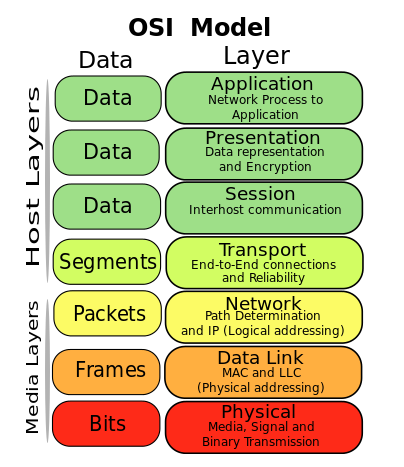
\includegraphics[height=5cm, width=5cm, keepaspectratio=true]{./images/Osi-model-jb}}

    \end{frame}

    %\framedgraphic{7 Layer Model}{./images/Osi-model-jb}
    
    \begin{frame}{CAN as Foundation}
      \begin{block}{Layers 1 and 2}
        From the bottom up, a CAN network needs to be looked at in terms of its physical implementation. We will consider the Physical (L1) and Data Link (L2) layers.
      \end{block}
      \centering{  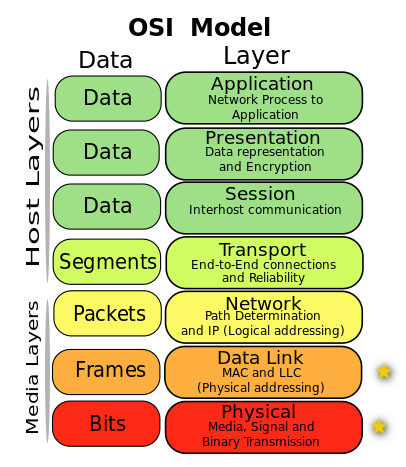
\includegraphics[height=4cm, width=4cm, keepaspectratio=true]{./images/Osi-model-jb-can}}
\end{frame}


    \framedgraphic{Network}{./images/generic_network}

    \framedgraphic{Exchange}{./images/can_signaling}

    \framedgraphic{Signaling Example}{./images/dso-can}
    
    \framedgraphic{Messages}{./images/CAN-Bus-frame_in_base_format_without_stuffbits}

    \begin{frame}{Theory to Practice}
      To implement the hardware of a CAN-based device, we need to provide the L1 and L2 features.\\
      Two Options:
      \begin{enumerate}
      \item{Use a standalone IC that covers both L1 and L2 requirements $OR$}
      \item{Use an SoC/MCU with built in CAN module (L2) and possibly a transceiver IC (L1)}
      \end{enumerate}
      \end{frame}

      \begin{frame}{Example - Standalone IC}
        \huge{Microchip MCP2515}
        \centering
            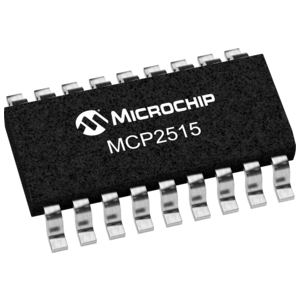
\includegraphics[height=5cm, width=5cm, keepaspectratio=true]{./images/mcp2515_pic}
      \end{frame}

      
     \framedgraphic{Example - MCP2525}{./images/mcp2515_blockdiagram}

     \framedgraphic{Hardware Solution with MCP2525}{./images/mcp2525_soln}

     \begin{frame}{Example - Use Integrated L2 CAN with L1 Transceiver}
        \huge{Texas Instruments ISO1050 Isolated CAN Transceiver}
        \centering
            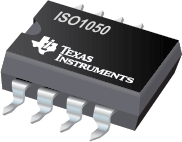
\includegraphics[height=5cm, width=5cm, keepaspectratio=true]{./images/ISO1050}
     \end{frame}

     \framedgraphic{Example - TI ISO1050}{./images/ISO1050_blockdiagram}
     
     \framedgraphic{Solution with ISO1050}{./images/ISO1050_soln}
     \section{Cometh the Protocols}
     \begin{frame}{Moving up the Stack}
       \huge
       \textbf{Q: What to do with all this reliable L1 and L2 infrastructure?}\\\pause
       A: Write standards of how our devices will use it!
     \end{frame}

     \begin{frame}{Horses for Courses}
       Some examples of the protocols using CAN as a foundation:
       \begin{description}
       \item[J1939] \textbf{1990} Control in heavy machinery e.g. Trucks,  Tractors. Created and governed by SAE. Baud rate of 250kbit/s, up to 30 nodes.
         \pause
       \item[DeviceNet] \textbf{1992} Industrial control. Created by Allen Bradley, eventually governed by ODVA. Baud rate of 125/250/500kbits/s, up to 64 nodes.
         \pause
         \item[CANopen] \textbf{1994} Industrial control. Created/governed by CiA. Up to 1Mbit/s, up to 127 nodes.
       \end{description}
     \end{frame}

     \begin{frame}
       How come all these protocols?\pause
       \begin{itemize}
       \item{Purpose}\pause
       \item{Flexibility}\pause
       \item{Implementation}
       \end{itemize}
     \end{frame}

     \begin{frame}{CANopen Protocol}
       \begin{quotation}
         CANopen provides several communication objects, which enable device designers to implement desired network behavior into a device. With these communication objects, device designers can offer devices that can communicate process data, indicate device-internal error conditions or influence and control the network behavior.
         \end{quotation}
       
       \end{frame}
       
     
%% % Empty Template
%% \begin{frame}
%%     \frametitle{}
%%     \framesubtitle{}
%%     %content goes here
%%   \end{frame}


}
\end{document}

